\subsection*{Section4.3}
\textbf{Problem 3}
The roots are 
\[
    r^2- 6r + 10 
    \implies r = \frac{6 \pm \sqrt{36-40}}{2}
    \implies r = 3 \pm i
\]
The general solution is
\[
    y = c_1e^{3t}\cos t + c_2e^{3t}\sin t
\]
\textbf{Problem 6}
The roots are 
\[
    r^2-4r+7
    \implies r = \frac{4 \pm \sqrt{16-28}}{2}
    \implies r = 2 \pm \sqrt{3}i
\]
The general solution is 
\[
    y = c_1e^{2t}\cos (\sqrt{3}t) + c_2e^{2t}\sin (\sqrt{3}t)
\]
\textbf{Problem 17}
The roots are 
\[
    r^2-r+7 = 0 
    \implies r = \frac{1 \pm \sqrt{1-28}}{2}
    \implies r = \frac{1}{2} \pm \frac{3\sqrt{3}}{2}
\]
The general solution is 
\[
    y = c_1e^{\frac{t}{2}}\cos (\frac{3\sqrt{3}t}{2}) + 
        c_2e^{\frac{t}{2}}\sin (\frac{3\sqrt{3}t}{2})
\]
\textbf{Problem 24}
The roots are 
\[
    r^2 + 9 = 0
    \implies r = 3i
\]
The general solution is 
\[
    y = c_1\cos 3t + c_2\sin 3t
\]
At the initial conditions,
\[
    1 = c_1
\]
\[
    1 = 3c_2
\]
The final solution is 
\[
    y = \cos 3t + \frac{1}{3}\sin 3t
\]
\textbf{Problem 25}
The roots are 
\[
    r^2 - 2r + 2 = 0
    \implies r = \frac{2 \pm \sqrt{4-8}}{2}
    \implies r = 1 \pm i
\]
The general solution is 
\[
    y = c_1e^t\cos t + c_2e^t\sin t
\]
At the initial conditions,
\[
    e^\pi = -c_1e^\pi 
\]
\[
    0 = c_1e^\pi-c_2e^\pi
\]
The final solution is 
\[
    y = e^t\sin t - e^t\cos t
\]
\textbf{Problem 26}
The roots are 
\[
    r^2 - 2r + 1 = 0
    \implies r = \frac{2 \pm \sqrt{4-4}}{2}
    \implies r = 1
\]
The general solution is 
\[
    y = c_1e^t + c_2te^t
\]
At the initial conditions,
\[
    1 = c_1 
\]
\[
    -2 = c_1 + c_2
\]
The final solution is 
\[
    y = e^t - 3te^t
\]
\textbf{Problem 28}
The roots are 
\[
    r^2 + br + 4 = 0
    \implies r = \frac{-b \pm \sqrt{b^2-16}}{2}
\]
For $b=5$,
\[
    r_5 = -\frac{5}{2} \pm \frac{3}{2}
    \implies r_5 = -4, -1
\]
The general solution is 
\[
    y_5 = c_1e^{-4t} + c_2e^{-t}
\]
At the initial conditions,
\[
    1 = c_1 + c_2
\]
\[
    0 = -4c_1 - c_2
\]
The final solution is 
\[
    y_5 = -\frac{1}{3}e^{-4t} + \frac{4}{3}e^{-t}
\]
For $b=4$,
\[
    r_4 = -2
\]
The general solution is 
\[
    y_4 = c_1e^{-2t} + c_2te^{-2t}
\]
At the initial conditions,
\[
    1 = c_1 
\]
\[
    0 = -2c_1 + c_2
\]
The final solution is 
\[
    y_4 = e^{-2t} + 2te^{-2t}
\]
For $b=2$,
\[
    r_2 = -1 \pm \sqrt{3}i
\]
The general solution is 
\[
    y_2 = c_1e^{-t}\cos \sqrt{3}t + c_2e^{-t}\sin \sqrt{3}t
\]
At the initial conditions,
\[
    1 = c_1
\]
\[
    0 = -c_1 + \sqrt{3} c_2
\]
The final solution is 
\[
    y_2 = e^{-t}\cos \sqrt{3}t + \frac{1}{\sqrt{3}}e^{-t}\sin \sqrt{3}t
\]
Graphing the equations yields
(not quite sure why $b=2$ graph isn't working),

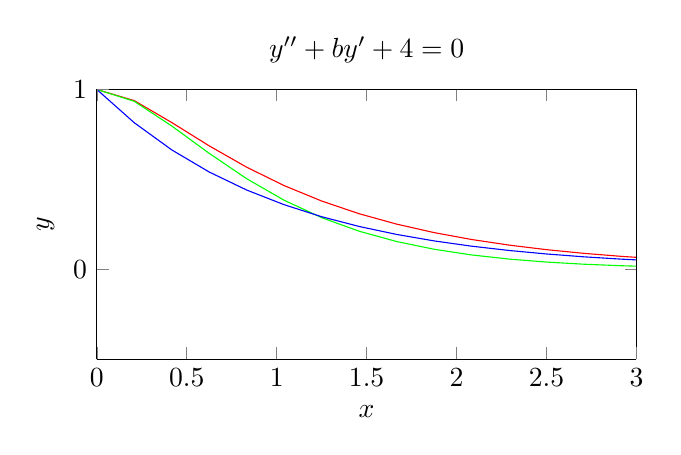
\begin{tikzpicture}
    \begin{axis}[
        xmin = 0, xmax = 3,
        ymin = -0.5, ymax = 1,
        zmin = 0, zmax = 1,
        axis equal image,
        view = {0}{90},
        title = {$y''+by'+4=0$},
        xlabel = {$x$},
        ylabel = {$y$},
    ]
    \addplot[red, domain=0:5]{-e^(-4*x)/3 + 4*e^(-x)/3};
    \addplot[green, domain=0:5]{e^(-2*x)+2*x*e^(-2*x)};
    \addplot[blue, domain=-0:5]{e^(-x)*(cos(sqrt(3)*x) + sin(sqrt(3)*x)/sqrt(3))};
    
    \end{axis}
\end{tikzpicture}
